\documentclass{article}
\usepackage[utf8]{vietnam}
\usepackage[11pt]{extsizes}
\usepackage{amsmath,amsfonts,amsthm}
\usepackage{geometry}
\usepackage{mathrsfs}
\usepackage{graphicx}
\usepackage{float}
 \geometry{
 a4paper,
 total={170mm,257mm},
 left=20mm,
 top=20mm,
}
\usepackage{enumitem} 
\title{Chuỗi Fourier và biến đổi Fourier}
\begin{document}
\maketitle
\section{Chuỗi Fourier}
\subsection{Định nghĩa chuỗi Fourier}
Một tín hiệu tuần hoàn bất kì có thể được biểu diễn bằng tổng của nhiều tín hiệu sine và cosine với các tần số khác nhau.
\subsection{Điều kiện tồn tại chuỗi FS (điều kiện Dirichlet)}
Điều kiện để một tín hiệu tuần hoàn có thể được biểu diễn bởi một chuỗi Fourỉer là:
\begin{equation*}
    \int_{T}|x(t)|dt < +\infty
\end{equation*}
\begin{equation*}
    \sum_{n=<N_{0}>}|x[n]|<+\infty
\end{equation*}
\subsection{Công thức chuỗi FS liên tục (CTFS)}
\begin{equation*}
    x(t)=\sum_{k=-\infty}^{+\infty}a_{k}e^{jk\omega_{0} t}
\end{equation*}
\begin{equation*}
    X[k] = a_{k}=\frac{1}{T}\int_{T}x(t)e^{-jk\omega_{0} t}dt
\end{equation*}
2 cặp công thức này luôn đi song song với nhau và gọi là CTFS pair. Các cách kí hiệu $X[k]$, $a_{k}$ hay $c_{k}$ đều có cùng một ý nghĩa là để chỉ hệ số chuỗi Fourier, tùy vào từng sách khác nhau thôi. Anh thích kí hiệu $a_{k}$ hơn vì nó hợp lý và đỡ lẫn hơn.
\subsection{Công thức chuỗi FS rời rạc (DTFS)}
$$x[n]=\sum_{k=<N_{0}>}c_{k}e^{jk\Omega_{0}n}$$
$$X[k]=c_{k}=\frac{1}{N_{0}}\sum_{n=<N_{0}>}x[n]e^{-jk\Omega_{0}n}$$
2 cặp công thức này luôn đi song song với nhau và gọi là DTFS pair.
\subsection{Bài tập}
\subsubsection{Dạng 1: Xác định hệ số chuỗi CTFS}
Bài 1: $$x(t)=\sin{\left(\frac{\pi}{3}-\frac{\pi}{2}\right)}+2\cos{\left(\frac{\pi}{2}t\right)}$$
\\Dạng bài này thì chỉ cần áp dụng thẳng công thức Euler vào là xong.
\begin{equation*}
    \begin{split}
x(t)&=\sin{\left(\frac{\pi}{3}t-\frac{\pi}{2}\right)}+2\cos{\left(\frac{\pi}{2}t\right)}\\&=\frac{1}{2j}(e^{j(\frac{\pi}{3}t-\frac{\pi}{2})}-e^{-j(\frac{\pi}{3}t-\frac{\pi}{2})})+e^{j\frac{\pi}{2}t}+e^{-j\frac{\pi}{2}t}
 \\ &=\frac{1}{2j}e^{-j\frac{\pi}{2}}e^{j\frac{\pi}{3}}-\frac{1}{2j}e^{j\frac{\pi}{2}}e^{-j\frac{\pi}{3}}+e^{j\frac{\pi}{2}t}+e^{-j\frac{\pi}{2}t}
\\&=\frac{1}{2j}e^{-j\frac{\pi}{2}}e^{j2\omega_{0}t}-\frac{1}{2j}e^{j\frac{\pi}{2}}e^{-j2\omega_{0}t}+e^{j3\omega_{0}t}+e^{-j3\omega_{0}t}
    \end{split}
\end{equation*}
Vậy ta có các hệ số $a_{k}$ như sau:
\begin{equation*}
a_{2}=\frac{1}{2j}e^{-j\frac{\pi}{2}}=\frac{-1}{2}, a_{-2}=-\frac{1}{2j}e^{j\frac{\pi}{2}}=\frac{-1}{2},a_{3}=a_{-3}=1
\end{equation*}
Vậy ta tìm được công thức khai triển chuỗi FS là: $$X[k]=\frac{-1}{2}\delta[k-2]-\frac{1}{2}\delta{[k+2]}+\delta{[k-3]}+\delta{[k+3]}$$
\\ Làm tương tự với các bài còn lại:
\\ Bài 2: 
$$x(t)=3\cos{\left(\frac{\pi}{2}t+\frac{\pi}{4}\right)}$$
Đáp án:
\begin{equation*}
X[k]= \begin{cases}
\frac{3}{2}e^{j\frac{\pi}{4}} &\ (k=1)\\
\frac{3}{2}e^{-j\frac{\pi}{4}} &\ (k=-1)\\
 0 &\ \text{(otherwise)}\\
\end{cases}
\end{equation*}
Bài 3:
$$x(t)=\sin{(2t)}-3\cos{(3t+1)}+1$$
Đáp án:
$$X[k]=\delta[k]-\frac{j}{2}\delta{[k-2]}+\frac{j}{2}\delta{[k+2]}-\frac{e^{j}}{2}\delta{[k-3]}-\frac{e^{-j}}{2}\delta{[k+3]}$$
\subsubsection{Dạng 2: Xác định hệ số chuỗi DTFS}
Bài 1: $$x[n]=\sum_{m=-\infty}^{+\infty}\delta{[n-3m+1]}$$
\\Dạng này chỉ cần thuộc công thức và vẽ hình là sẽ làm được. Với câu trên, ta vẽ hình và nhìn thấy $N_{0}=3$, vậy ta có:
$$c_{k}=\frac{1}{N_{0}}\sum_{n=<N_{0}>}x[n]e^{-jk\Omega_{0}n}=\frac{1}{3}\sum_{n=-2}^{0}x[n]e^{-jk\Omega_{0}n}=\frac{1}{3}e^{jk\frac{2\pi}{3}}$$
Ở đây ta chọn khoảng $n$ chạy từ $-2\to0$ (đi qua $3$ điểm, nhưng cũng có thể chọn các khoảng khác như $0\to 2$ cũng tính ra cùng một kết quả, miễn là nó đi qua $N_{0}$ điểm)
\\Bài 2: $$x[n]=\sum_{m=-\infty}^{+\infty}\delta{[n-3m]}$$
Đáp án: $$X[k]=\frac{1}{3}$$
\\ Bài 3: Tín hiệu $x[n]$ có chu kì cơ sở tuần hoàn $N_{0}=10$ và một chu kì được biểu diễn như sau:
\begin{equation*}
    x[n]=
    \begin{cases}
        1 &\ (n=0)\\
        -1  &\ (n=8)\\
        0 &\ (\text{otherwise})\\
    \end{cases}
\end{equation*}
Đáp án:
$$X[k]=\frac{1}{10}\left(1-e^{-j\frac{2\pi}{5}k}\right)$$
\subsubsection{Dạng 3: Xác định hệ số chuỗi CTFS từ một tín hiệu bất kì}
Dạng bài này tương đối dễ chỉ cần dùng đúng công thức, anh nghĩ chỉ cần học dạng bài này với trường hợp duy nhất đầu vào xung chữ nhật là được. 
\\ Xác định các hệ số chuỗi Fourier của tín hiệu $x(t)$ tuần hoàn với chu kì $T_{0}=2(s)$ và một chu kì được biểu diễn như sau:
\begin{equation*}
    x(t)=
    \begin{cases}
        1 &\ (0\leq t<1)\\ 0 &\ (1\leq t <2) \\
    \end{cases}
\end{equation*}
Ta dùng công thức:
\begin{equation*}
    \begin{split}
    a_{k}&=X[k]=\frac{1}{T_{0}}\int_{T_{0}}x(t)e^{-jk\omega_{0}t}dt=\frac{1}{2}\int_{0}^{1}e^{-jk\omega_{0}t}dt=-\frac{1}{2}\frac{e^{-jk\omega_{0}t}}{jk\omega_{0}}\Big|_0^1=\frac{1-e^{-jk\omega_{0}}}{j2k\omega_{0}}\\&=\frac{1-e^{-jk\pi}}{j2k\pi}
    \end{split}
\end{equation*}
Các dạng nâng cao hơn như xung tam giác, xung răng cưa thì anh không nghĩ thầy cho khó đến mức đấy đâu.
\subsubsection{Dạng 4: Xác định hệ số chuỗi CTFS từ đồ thị}
Như anh đã nói, đây là dạng bài rất trọng tâm và phải cày nhiều dạng này. Anh sẽ lấy ví dụ một câu và các câu khác tự tìm lại trong đống Quiz và làm tương tự.
\begin{figure}[H]
\centering
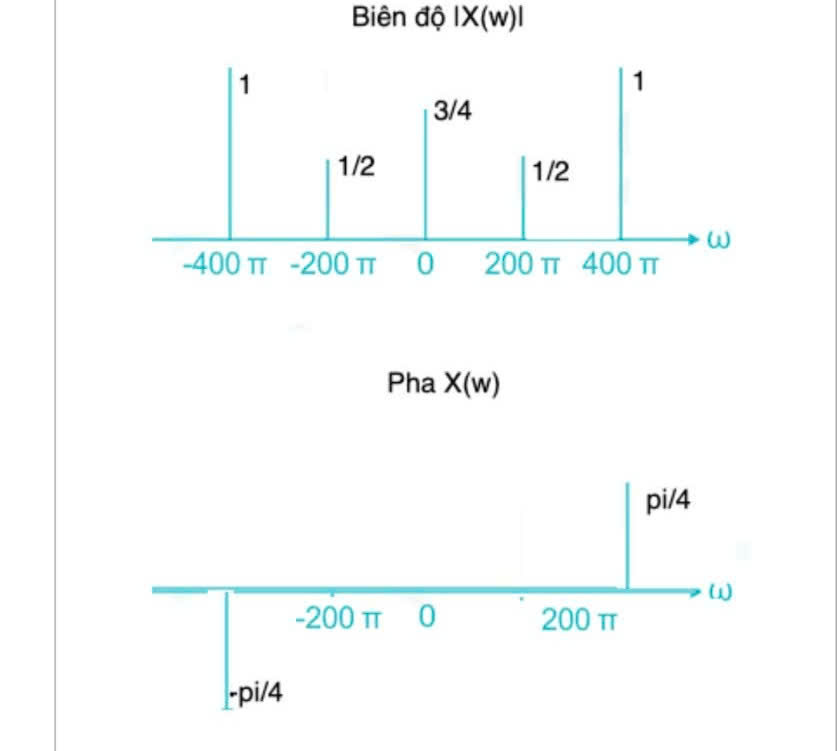
\includegraphics[width=0.5\textwidth]{fs.jpg}
\caption{Đồ thị phổ pha và phổ biên độ của tín hiệu gốc $x(t)$}
\end{figure}
Từ đồ thị phổ biên độ và pha, ta xác định lại được các hệ số chuỗi CTFS như sau:
\begin{equation*}
    \begin{cases}
        a_{0}=\frac{3}{4}\\
        a_{1}=a_{-1}=\frac{1}{2}\\
        a_{2}=e^{j\frac{\pi}{4}}\\
        a_{-2}=e^{-j\frac{\pi}{4}}\\
    \end{cases}
\end{equation*}
Với tần số góc cơ sở $\omega_{0}=200\pi$, ta khôi phục lại được tín hiệu như sau:
\begin{equation*}
    \begin{split}
    x(t)&=\sum_{k=-\infty}^{+\infty}a_{k}e^{jk\omega_{0}t}=\frac{3}{4}+\frac{1}{2}e^{j\omega_{0}t}+\frac{1}{2}e^{-j\omega_{0}t}+e^{j\frac{\pi}{4}}e^{j2\omega_{0}t}+e^{-j\frac{\pi}{4}}e^{-j2\omega_{0}t}\\&=\frac{3}{4}+\cos{(\omega_{0}t)}+2\cos{\left(2\omega_{0}t+\frac{\pi}{4}\right)}=\frac{3}{4}+\cos{(200\pi t)}+2\cos{\left(400\pi t+\frac{\pi}{4}\right)}
    \end{split}
\end{equation*}
\subsubsection{Dạng 5: Khôi phục tín hiệu từ các hệ số chuỗi DTFS}
Đây là dạng toán "ngược" của dạng toán tìm hệ số chuỗi DTFS. Nhìn chung cách giải thì cứ tách lại theo công thức Euler là xong.
\\ Bài 1: Khôi phục một chu kì tín hiệu gốc $x[n]$ $(-5\leq n\leq 5)$ từ chuỗi DTFS sau:
\\ Do một chu kì chạy từ $-5\leq n\leq 5$, nên ta thấy $N_{0}=11$, vậy tần số góc cơ sở của tín hiệu là $\Omega_{0}=\frac{2\pi}{N_{0}}=\frac{2\pi}{11}$
\begin{equation*}
    \begin{split}
X[k]&=\cos{\left(\frac{4\pi}{11}k\right)}+2j\sin{\left(\frac{6\pi}{11}k\right)}=\frac{1}{2}e^{j\frac{4\pi}{11}k}+\frac{1}{2}e^{-j\frac{4\pi}{11}k}+e^{j\frac{6\pi}{11}k}-e^{-j\frac{6\pi}{11}k}\\&=\frac{1}{2}e^{j2\Omega_{0}k}+\frac{1}{2}e^{-j2\Omega_{0}k}+e^{j3\Omega_{0}k}-e^{-j3\Omega_{0}k}
    \end{split}
\end{equation*}
Vậy ta suy ra công thức của tín hiệu gốc trong một chu kì là:
$$x[n]=\frac{1}{2}\delta{[n-2]}+\frac{1}{2}\delta{[n+2]}+\delta{[n-3]}-\delta{[n+3]}$$
Bài 2: Khôi phục lại một chu kì tín hiệu gốc $N_{0}=6$ với $0\leq k \leq5$ từ chuỗi DTFS sau:
$$X[k]=\delta{[k-2]}-2\delta{[k-3]}+\delta{[k-4]}$$
Đáp án: 
$$x[n]=2\cos{\left(\frac{2\pi}{3}n\right)}-2\cos{(\pi n)}$$
\subsubsection{Dạng 6: Khôi phục tín hiệu từ các hệ số chuỗi CTFS}
Bài 1: Khôi phục tín hiệu $x(t)$ có chu kì cơ sở $T_{0}=2(s)$ và có hệ số chuỗi sau:
$$X[k]=-j\delta{[k-2]}+j\delta{[k+2]}+2\delta{[k-3]}+2\delta{[k+3]}$$
Từ chuỗi $X[k]$ ta có thể thấy ngay các hệ số chuỗi tương ứng là:
\begin{equation*}
    \begin{cases}
        a_{2}=-j \\
        a_{-2}=j\\
        a_{3}=2\\
        a_{-3}=2\\
    \end{cases}
\end{equation*}
Do chu kì cơ sở của tín hiệu là $T_{0}=2(s)$, nên suy ra $\omega_{0}=\pi$, ta xây dựng công thức tìm lại tín hiệu $x(t)$ gốc:
\begin{equation*}
    \begin{split}
x(t)&=\sum_{k=-\infty}^{+\infty}a_{k}e^{jk\omega_{0}t}=-je^{j2\pi t}+je^{-j2\pi t}+2e^{j3\pi t}+2e^{-j3\pi t}\\&=-j(e^{j2\pi t}-e^{-j2\pi t})+2(e^{j3\pi t}+e^{-j 3\pi t})=2\sin{(2\pi t)}+4\cos{(3\pi t)}
    \end{split}
\end{equation*}
Bài 2: Khôi phục tín hiệu $x(t)$ có chu kì cơ sở $T_{0}=6(s)$ và có hệ số chuỗi sau:
$$X[k]=\delta{[k+2]}+\delta{[k-2]}+2j\delta{[k+3]}-2j\delta{[k-3]}$$
Đáp án: $$x(t)=2\cos{\left(\frac{2\pi t}{3}\right)}+4\sin{(\pi t)}$$
\subsubsection{Dạng 7: Tìm đáp ứng của hệ thống LTI với đầu vào tín hiệu tuần hoàn}
Đây là dạng bài chắc là khó và cũng là quan trọng nhất của phần FS rồi, lưu ý ôn kĩ dạng này để thi cuối kì học cho đỡ khổ vì đây là dạng câu hỏi mà gần như đề tự luận nào cũng có.
\\ Dạng này để lại để đến lúc live thì anh sẽ dạy sau.
\section{Biến đổi Fourier}
\subsection{Định nghĩa biến đổi Fourier}
Biến đổi Fourier là dạng tổng quát hơn của chuỗi FS, khi mà các chu kì $T_{0}$ hay $N_{0}$ tiến ra dương vô cùng. Có thể hiểu một cách đơn giản là biến đổi Fourier (Fourier Transform) là biến đổi dùng cho
các tín hiệu \textbf{không tuần hoàn tổng quát}, tức là tương đương với chu kì tuần hoàn bằng dương vô cực, hơi trừu tượng nhưng cố tưởng tượng chút là hiểu.
\subsection{Điều kiện tồn tại FT}
Một tín hiệu có thể biến đổi Fourier được khi và chỉ khi nó là một \textbf{tín hiệu năng lượng}, tức là năng lượng của nó trên toàn miền thời gian là hữu hạn.
$$\int_{-\infty}^{+\infty}|x(t)|^2dt < + \infty$$
$$\sum_{n=-\infty}^{+\infty}|x[n]|^2 < + \infty$$
\subsection{Công thức biến đổi Fourier cho tín hiệu liên tục CTFT}
Tương tự như trên, ta cũng có công thức CTFT pair cho tín hiệu liên tục:
$$x(t)=\frac{1}{2\pi}\int_{-\infty}^{+\infty}X(\omega)e^{j\omega t}d\omega$$
$$X(\omega)=\int_{-\infty}^{+\infty}x(t)e^{-j\omega t}dt$$
Theo như anh thấy thì đa phần công thức $x(t)$ chỉ dùng để chứng minh các tính chất của biến đổi Fourier chứ chưa bao giờ dùng làm bài tập cả, nên công thức này có thể không nhớ cũng được, nhưng công thức $X(\omega)$ thì bắt buộc phải nắm rất rõ.
\subsection{Tính chất của CTFT}
CTFT có khoảng 10 tính chất cần phải thuộc, gồm:
\begin{enumerate}
    \item 
\end{enumerate}
\subsection{Công thức biến đổi Fourier cho tín hiệu rời rạc DTFT}
Công thức biến đổi Fourier cho tín hiệu rời rạc như sau:
$$x[n]= $$
\subsection{Bài tập}
\subsubsection{Dạng 1: Tính CTFT của các tín hiệu sau}
Áp dụng công thức $X(\omega)$ để tìm FT của các tín hiệu sau:
\begin{itemize}
    \item $$x(t)=e^{-|t-1|}$$
    \item $$x(t)=e^{2t}[u(t)-u(t-1)]$$
    \item $$x(t)=e^{-at}u(t) \quad(a>0)$$
    \item $$x(t)=e^{at}u(-t) \quad(a>0)$$
\end{itemize}
Tự tra bảng công thức "Common Continuous Time Fourier Transform Pairs" và cố gắng chứng minh lại càng nhiều công thức càng tốt.
\end{document}
